%%%%%%%%%%%%%%%%%%%%%%%%%%%%%%%%%%%%%%%%%
% University/School Laboratory Report
% LaTeX Template
% Version 3.1 (25/3/14)
%
% This template has been downloaded from:
% http://www.LaTeXTemplates.com
%
% Original author:
% Linux and Unix Users Group at Virginia Tech Wiki 
% (https://vtluug.org/wiki/Example_LaTeX_chem_lab_report)
%
% License:
% CC BY-NC-SA 3.0 (http://creativecommons.org/licenses/by-nc-sa/3.0/)
%
%%%%%%%%%%%%%%%%%%%%%%%%%%%%%%%%%%%%%%%%%

%----------------------------------------------------------------------------------------
%	PACKAGES AND DOCUMENT CONFIGURATIONS
%----------------------------------------------------------------------------------------

\documentclass{article}

\usepackage{graphicx} % Required for the inclusion of images
\usepackage{natbib} % Required to change bibliography style to APA
\usepackage{amsmath} % Required for some math elements 
\usepackage{polski}
\usepackage{hyperref}
\usepackage{listings}
\usepackage{sidecap}
\usepackage{outlines}
\graphicspath{ {./images/}}
\usepackage[utf8]{inputenc}
\setlength\parindent{0pt} % Removes all indentation from paragraphs

\renewcommand{\labelenumi}{\alph{enumi}.} % Make numbering in the enumerate environment by letter rather than number (e.g. section 6)

%\usepackage{times} % Uncomment to use the Times New Roman font

%----------------------------------------------------------------------------------------
%	DOCUMENT INFORMATION
%----------------------------------------------------------------------------------------

\title{Stacja zliczająca przejeżdzające rowery \\ przy użyciu STM32 F3 Discovery \\ Systemy Wbudowane 2019} % Title

\date{23 X 2019} % Date for the report

\begin{document}

\maketitle % Insert the title, author and date

\begin{center}
Marcin Pajkowski 211968 (Kierownik)\\ % Partner names
Bartosz Myśliwiec 211827 \\
\end{center}

% If you wish to include an abstract, uncomment the lines below
% \begin{abstract}
% This paper describes 
% \end{abstract}

%----------------------------------------------------------------------------------------
%	Listę wykorzystanych funkcjonalności;
%----------------------------------------------------------------------------------------

\section{Lista wykorzystanych funkcjonalności}

Protokoły wejścia/wyjścia:
\begin{itemize}
    \item General-purpose I/O,
    \item Serial Peripheral Interface,
    \item Nested Vectorized Interrupt Controller,
    \item Universal Asynchronous Receiver-Transmitter.
\end{itemize}

Urządzenia zewnętrzne:
\begin{itemize}
    \item znajdujące się na MCU diody LED,
    \item wyświetlacz,
    \item czujnik zbliżeniowy typu PIR,
    \item moduł Bluetooth.
\end{itemize}

 
%----------------------------------------------------------------------------------------
%	Zakres obowiązków każdego z Autorów (czyli co zrobił?) 
% 	wraz z zaproponowanym przez kierownika projektu udziałem  %	pracy.
%----------------------------------------------------------------------------------------

\newpage
\section{Zakres obowiązków}

\begin{tabular}{|l|l|}
    \hline
    Osoba odpowiedzialna & Moduł funkcjonalny\\
    \hline
    Marcin Pajkowski
    & Przygotowanie środowiska pracy (IDE, repozytorium Git)\\
    & Komunikacja UART (serial.h, serial.c)\\
    & Sygnalizacja za pomocą diod (led.h, led.c)\\
    & Moduł logujący (trace.h)\\
    & Czujnik ruchu (motion.h, motion.c)\\
    \hline
    Bartosz Myśliwiec
    & RTC\\
    & Wyświetlacz (display.h, display.c)\\
    & Czujnik temperatury (display.h, display.c)\\
    & Przycisk (button.h, button.c)\\
    \hline
\end{tabular}

%----------------------------------------------------------------------------------------
%	Opis działania programu 
%----------------------------------------------------------------------------------------

\section{Opis działania programu}
\subsection{Instrukcja użytkownika}

Urządzenie umożliwi wymianę komunikatów za pomocą interfejsu UART. Odbiorca urządzenia
musi upewnić się, że jego komputer posiada możliwość komunikacji. W systemach
z rodziny GNU/Linux może okazać się konieczne posiadanie uprawnienia do tworzenia
procesów jako użytkownik uprzywilejowany lub przynależność do grupy dialout.

Od momentu włączenia/resetu wysyłane jest do portu szeregowego informacja o zarejestrowanym
ruchu. Ramka danych ma następującą postać:

\begin{lstlisting}
    +DATABEGIN+[data];[czas]+DATAEND+\r\n
\end{lstlisting}

przy czym pole \emph{data} ma format \emph{DD.MM.YYYY}, a pole czas - \emph{HH:MM:SS} (format 24-godzinny).

Zastosowanie ramki umożliwia odfiltrowanie informacji o zdarzeniu ruchu od logów, które
są wysyłane za pomocą tego samego UART.

\subsection{Korzystanie z komend powłoki}
Za pomocą interfejsu UART możemy wysyłać komendy do rejestratora ruchu. Ogólna postać komendy
prezentuje się następująco:

\begin{lstlisting}
    komenda [argumenty,...]
\end{lstlisting}

Wprowadzone dane należy zatwierdzić używając znaku '='.

\subsubsection{Ustawianie daty}
W celu ustawienia daty należy użyć komendy \emph{setDate} w następujący sposób:

\begin{lstlisting}
    setDate DD,MM,YYYY
\end{lstlisting}

\subsubsection{Ustawianie czasu}
W celu ustawienia czasu należy użyć komendy \emph{setTime} w następujący sposób:

\begin{lstlisting}
    setTime HH,SS
\end{lstlisting}

\subsubsection{Pobieranie informacji o aktualnym czasie}
Aby otrzymać informacje o aktualnym czasie należy użyć komendy \emph{getTime}:

\begin{lstlisting}
    getTime
\end{lstlisting}

\subsubsection{Pobieranie informacji o aktualnej dacie}
Aby otrzymać informacje o aktualnej dacie należy użyć komendy \emph{getDate}:

\begin{lstlisting}
    getDate
\end{lstlisting}

% TODO - przykłady odpowiedzi rejestratora

\subsection{Opis algorytmu}

\subsubsection{Ogólny opis algorytmu}
Po włączeniu urządzenia wywoływane są funkcje inicjalizujące moduły funkcjonalne
urządzenia. Podczas tego procesu konfigurowane i włączane zostają porty GPIO,
peryferia odpowiadające za I/O, kontrolery przerwań oraz zegary.

Od momentu włączenia urządzenie oczekuje na komunikat z czujnika PIR o wykrytym ruchu - sygnalizowany
jest on wystawieniem stanu wysokiego na wyjściu GPIO związanego z tym czujnikiem.

%----------------------------------------------------------------------------------------
%	Opis działania wykonanego sprzętu wraz z notami 	  	katalogowymi (w dodatkowych plikach) z wyjaśnieniem dlaczego zrobione jest tak, a nie inaczej.
%Jeżeli nie było wykonanego sprzętu, to trzeba napisać, że %nie było;
%----------------------------------------------------------------------------------------

\section{Opis działania wykonanego sprzętu wraz z notami katalogowymi}

\subsection{Moduł główny}
% TODO: GPIO, UART, SPI, RTC, EXTI, NVIC
Projekt został zrealizowany z użyciem płytki ewaluacyjnej STM32F3 Discovery.
Układ ten został wyposażony w procesor rodziny Arm® Cortex®-M4 - STM32F303VCT6.

\subsubsection{Datasheet}
\url{https://www.st.com/resource/en/data_brief/stm32f3discovery.pdf}
\newline
\url{https://www.st.com/resource/en/datasheet/stm32f303vc.pdf}

\subsection{Wyświetlacz PCD8544}

W projekcie został użyty monochromatyczny wyświetlacz ciekłokrystaliczny. Ten sam model
został użyty w telefonie Nokia 5110. Na wyświetlaczu prezentowany jest aktualny czas wraz z datą.
Komunikacja z wyświetlaczem jest zrealizowana za pomocą układu SPI.
Urządzenie w zakupionej przez nas wersji posiada 8 wyprowadzeń:

\begin{enumerate}
    \item RST - linia resetująca wyświetlacza,
    \item CE - linia NSS,
    \item DC - flaga trybu komend/danych,
    \item DIN - linia danych,
    \item CLK - linia SCK,
    \item VCC - zasilanie,
    \item BL - zasilanie podświetlenia,
    \item GND - masa.
\end{enumerate}

\subsubsection{Adresacja}
Rozdzielczość wyświetlacza to 84x48 pikseli. Ekran podzielony jest na 6 banków.
Taki podział ułatwia pracę z tekstem - po wysłaniu oktetu licznik adresów
X jest inkrementowany. W momencie osiągnięcia granicy wskaźnik X jest ustawiany na
0 a wskaźnik Y inkrementowany o 1. Dzięki takiemu sposobowi adresacji można użyć
jednowymiarowego bufora. W każdym bajcie najstarszy bit oznacza piksel znajdujący się najniżej,
zaś najmłodszy - piksel u góry.


\begin{figure}[ht]
    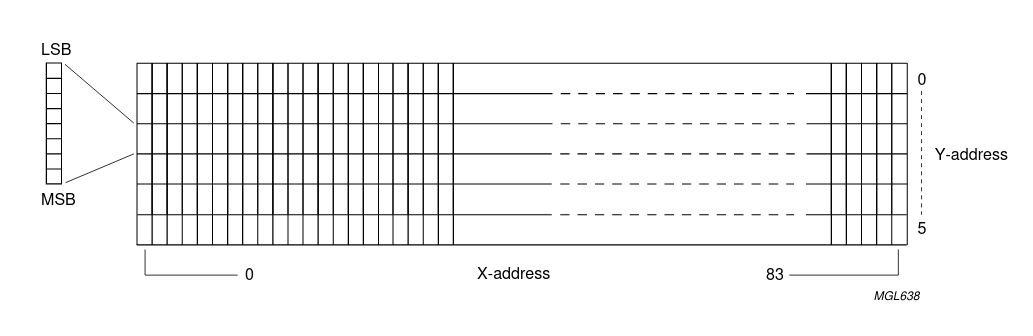
\includegraphics[scale=0.50]{address_display}
    \caption{Adresacja banków pamięci, V=0}
\end{figure}

\subsubsection{Inicjalizacja wyświetlacza}
Zaraz po włączeniu zasilania stany rejestrów i pamięci urządzenia są niezdefiniowane.
Należy wygenerować stan niski na linii RST. Następnie na tej samej linii ustawiany
jest stan wysoki.

\begin{center}
\begin{lstlisting}[language=C, basicstyle=\footnotesize]
void displayReset()
{
    LL_GPIO_ResetOutputPin(DISPLAY_PORT, DISPLAY_RST);
    LL_GPIO_SetOutputPin(DISPLAY_PORT, DISPLAY_RST);
} 
\end{lstlisting}
\end{center}

Następnie należy wysłać serię komend:

\begin{enumerate}
    \item Rozszerzony tryb komend
    \item Ustawienie kontrastu
    \item Współczynnik temperatury
    \item Współczynnik biasu
    \item Powrót do regularnego trybu komend
\end{enumerate}


\subsection{Wysyłanie komend/danych}
Aby wysłać do wyświetlacza komendę należy ustawić na linii DC stan wysoki. Wysyłanie danych
jest oznaczone stanem niskim.
\subsubsection{Datasheet}

\url{https://www.sparkfun.com/datasheets/LCD/Monochrome/Nokia5110.pdf}
\subsection{Czujnik ruchu}

\subsubsection{Opis}
Jako czujnik ruchu został wybrany czujnik typu PIR. Jest to urządzenie pasywne.
Czujniki tego typu wykrywają szybkie zmiany temperatury w swoim otoczeniu. Czujniki
PIR charakteryzują się wysoką ilością sygnałów \emph{false-positive}, dlatego też
urządzenie zastosowane w projekcie ma możliwość regulacji czułości, które pomaga
w znacznym stopniu zniwelować ten problem. Komunikacja z czujnikiem jest prosta - wystawia
on stan wysoki (+3V) na wyjściu w sytuacji, kiedy ruch zostanie wykryty.

\url{https://www.mpja.com/download/31227sc.pdf}
\subsection{Bluetooth}

Wybrane przez nas urządzenie umożliwia komunikację poprzez UART.

\url{http://www.electronicaestudio.com/docs/istd016A.pdf}

%----------------------------------------------------------------------------------------
% Opis funkcjonalności poszczególnych elementów, np. dla
% wejść wyjść cyfrowych w układach LPC należy opisać PINSEL
% (w używanym zakresie), IODIR, IOSET, IOCLR, IOPIN i tak dla
%  wszystkich używanych funkcjonalności [UART, SPI, I2C, PWM, ...]
% i interfejsów [Wyświetlacz, karta MMC/SD, Extender, karta sieciowa,
% akcelerometr, ...], czy przerwań (tych które są używane,
% dla LPC2xxx - FIQ,VIRQ,IRQ).
%----------------------------------------------------------------------------------------

\section{Opis funkcjonalności poszczególnych elementów}

Przycisk
\begin{itemize}
    \item AHB1
    \item GPIOA
    \begin{enumerate}
        \item PIN0 - Stan przycisku
    \end{enumerate}
\end{itemize}

Wyświetlacz
\begin{itemize}
    \item AHB1
    \item APB2
    \item SPI1
    \item GPIOA
        \begin{enumerate}
            \item PIN1 - DC
            \item PIN2 - Podświetlenie
            \item PIN4 - CE
            \item PIN5 - CLK
            \item PIN6 - Reset
            \item PIN7 - DIN
        \end{enumerate}
\end{itemize}

Diody LED
\begin{itemize}
    \item AHB1
    \item GPIOE - PIN8-PIN15 - stany diod LED
\end{itemize}

Czujnik ruchu
\begin{itemize}
    \item AHB1
    \item GPIOA
        \begin{enumerate}
            \item PIN3 - Odczyt stanu
        \end{enumerate}
\end{itemize}

Bluetooth
\begin{itemize}
    \item AHB1
    \item APB2
    \item USART1
    \item GPIOA
        \begin{enumerate}
            \item PIN9 - USART1 Transmitter
            \item PIN10 - USART1 Receiver
        \end{enumerate}
\end{itemize}


%----------------------------------------------------------------------------------------
%	BIBLIOGRAPHY
%----------------------------------------------------------------------------------------

\bibliographystyle{apalike}

\bibliography{sample}

%----------------------------------------------------------------------------------------


\end{document}